\documentclass[crop,tikz]{standalone}

\usetikzlibrary{automata, positioning, arrows}

\begin{document}
  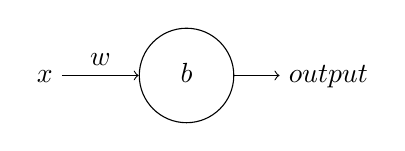
\begin{tikzpicture}[node distance=1.8cm]
    \tikzstyle{state}=[circle, draw, minimum size=1.2cm,inner sep=0]
    \tikzstyle{state io}=[line width=0]

    \node[state] (p) {\strut{$b$}};
    \node[state io, left of=p] (x) {\strut{$x$}};
    \node[state io, right of=p] (o) {\strut{$output$}};

    \path[->] (x) edge node[above] {$w$} (p);
    \path[->] (p) edge node {} (o);
  \end{tikzpicture}
\end{document}
